% Created 2026-04-12 Sun 08:12
% Intended LaTeX compiler: pdflatex
\documentclass[a4paper,11pt]{article}
\usepackage[utf8]{inputenc}
\usepackage[T1]{fontenc}
\usepackage{graphicx}
\usepackage{longtable}
\usepackage{wrapfig}
\usepackage{rotating}
\usepackage[normalem]{ulem}
\usepackage{amsmath}
\usepackage{amssymb}
\usepackage{capt-of}
\usepackage{hyperref}
\usepackage{longtable}
\usepackage{tabularx}
% --- Document metadata (must precede bv.sty which uses them in \hypersetup) ---
\newcommand{\bvReferenceNumber}{XXXXXX}
\newcommand{\bvIssue}{Pre}
\newcommand{\bvTitle}{Voyage Fuel Optimiser -- Software Architecture \& Validation}
\newcommand{\bvDate}{\today}
\newcommand{\bvType}{Technical Report}
\newcommand{\bvAuthor}{Frode Bloch}
\newcommand{\bvCompany}{Brunvoll AS}
\newcommand{\bvClassification}{INTERNAL}
\usepackage{/home/blofro/src/rdt_analysis/bv}
\usepackage{siunitx}
\sisetup{per-mode=symbol, inter-unit-product=\ensuremath{\cdot}}
\DeclareSIUnit{\knot}{kn}
\usepackage{amsmath}
\usepackage{subcaption}
\usepackage{eurosym}
\graphicspath{{images/}}
\author{Frode Bloch}
\date{\today}
\title{}
\hypersetup{
 pdfauthor={Frode Bloch},
 pdftitle={},
 pdfkeywords={},
 pdfsubject={},
 pdfcreator={Emacs 29.3 (Org mode 9.6.15)}, 
 pdflang={English}}
\begin{document}

\bvMainTitlePage
\tableofcontents
\newpage

\section{Introduction}
\label{sec:orgf2ee1fd}

This report documents the architecture and validation of the \texttt{voyage\_comparison}
propulsion optimiser tool.  The tool performs long-term hindcast-based voyage
simulations comparing the factory combinator pitch/RPM schedule against a
fuel-optimal operating point selection, with optional Flettner rotor
wind-assist.

The tool was originally implemented as a single 4\thinspace913-line Python
script.  A modular refactoring was carried out to improve maintainability,
testability, and extensibility.  This report describes the physical models, the
software architecture after refactoring, and presents validation results from a
full-year simulation on the Rotterdam--Gothenburg route.

\subsection{Scope}
\label{sec:orgbc42274}

The tool addresses the following question: \emph{for a given vessel on a fixed route,
how much fuel can be saved by optimising the propeller pitch and RPM at each
operating point, compared to the factory-default combinator schedule?}

The analysis chain covers:
\begin{itemize}
\item Calm-water hull resistance from model test data.
\item Wave added resistance via PdStrip drift transfer functions integrated over
JONSWAP spectra.
\item Blendermann (1994) wind resistance model.
\item Flettner rotor wind-assist thrust (Bordogna et al., 2019).
\item Hull and propeller roughness penalties (Townsin--Dey, 2003).
\item Factory combinator schedule replication.
\item Fuel-optimal pitch/RPM selection via propeller model optimisation.
\end{itemize}

Hindcast weather is provided by NORA3 (Norwegian Reanalysis Archive, 3\thinspace km
resolution) wave and wind fields.

\section{Physical Models}
\label{sec:org5de2acc}
\subsection{Hull Resistance}
\label{sec:org6fe67e8}

Calm-water resistance is interpolated from the vessel 206 model test trial
prediction (test 25-0461/25-0288, draught \SI{7.600}{\metre}, displacement
\SI{11165}{\metre\cubed}) at 15 speeds (\SIrange{8}{15.0}{\knot}).  No sea
margin removal is needed --- the resistance values are clean calm-water.  The
total thrust demand including environmental loads is:

\begin{equation}
  T_\text{prop} = \frac{R_\text{calm} + R_\text{aw} + R_\text{wind} + R_\text{rough} - F_\text{Flettner}}{1 - t}
\end{equation}

Wake fraction \(w(V_s)\) and thrust deduction \(t(V_s)\) are interpolated from
the self-propulsion test data.

\subsection{Wave Added Resistance}
\label{sec:org76c0b5f}

Wave added resistance is computed from PdStrip strip-theory transfer functions.
The \texttt{DriftTransferFunction} class loads the \texttt{.dat} output from PdStrip and
computes the mean surge drift force for a given sea state:

\begin{equation}
  R_\text{aw} = 2 \int_0^\infty S_\zeta(\omega;\, H_s, T_p)
                  \cdot C_\text{drift}(\omega,\, \theta_\text{rel})
                  \, d\omega
\end{equation}

where \(S_\zeta\) is the JONSWAP wave spectrum and \(C_\text{drift}\) is the
frequency- and heading-dependent drift force transfer function per unit wave
amplitude squared.

\subsection{Wind Resistance}
\label{sec:orgeb044fc}

Hull wind resistance follows Blendermann (1994), using tabulated surge force
coefficients \(C_X(\alpha)\) for a general cargo vessel:

\begin{equation}
  R_\text{wind} = -C_X(\alpha_\text{app}) \cdot \tfrac{1}{2}\,\rho_\text{air}\,
                   V_\text{app}^2 \cdot A_F
\end{equation}

where \(\alpha_\text{app}\) is the apparent wind angle from the bow, \(V_\text{app}\)
the apparent wind speed, and \(A_F = \SI{280}{\metre\squared}\) the frontal
projected wind area.

\subsection{Flettner Rotor}
\label{sec:orgb0af809}

The Flettner rotor model is ported from the BruCon C++ vessel simulator.  Lift
and drag coefficients follow Bordogna et al. (2019) with aspect-ratio correction
for a rotor of height \SI{28}{\metre} and diameter \SI{4}{\metre}:

\begin{itemize}
\item Lift and drag are tabulated as functions of spin ratio \(\text{SR} = \Omega R / V_\text{app}\).
\item The target spin ratio is \(\text{SR} = 3\) (max \SI{220}{RPM}).
\item Rotor drive power follows the Theodorsen \& Regier (1944) model.
\item Rotor motor fuel is charged at the auxiliary genset SFOC (\SI{215}{\gram\per\kilo\watt\hour}).
\end{itemize}

The net propulsive benefit is the surge component of the Magnus-effect force
minus the fuel penalty for driving the rotor.

\subsection{Hull and Propeller Roughness}
\label{sec:org0f7008f}

Hull roughness resistance follows Townsin \& Dey (2003):

\begin{equation}
  \Delta C_F = 0.044 \left[\left(\frac{k_s}{L}\right)^{1/3}
               - 10\,\text{Re}^{-1/3}\right] + 0.000125
\end{equation}

Propeller blade roughness increases torque (and thus fuel) via the empirical
model of Mosaad (1986).  Both roughness values can be specified directly in
\$\(\mu\)\$m or via a \texttt{FoulingScenario} which models piecewise-linear roughness growth
over time since last cleaning.

\subsection{Factory Combinator}
\label{sec:org59807d1}

The \texttt{FactoryCombinator} class replicates the BruCon vessel simulator's
\texttt{MakeNormalCombinator()} algorithm.  For a given thrust demand, it returns the
pitch and RPM dictated by the factory schedule---following the propeller curve up
to a break point, then constant RPM with increasing pitch.

\subsection{Propeller Model and Fuel Optimisation}
\label{sec:org5663a8f}

The fuel-optimal operating point is found by searching the full \((P/D,\, n)\)
space of the C-series propeller model.  For each thrust demand, the optimiser
finds the pitch/RPM combination that minimises engine SFOC \(\times\) brake power,
subject to the MAN L27/38 power envelope.

Results are pre-computed for a grid of 681 thrust values
(\SIrange{10}{350}{\kilo\newton} in \SI{0.5}{\kilo\newton} steps) using parallel
workers, then looked up during the voyage simulation for speed.

\section{Software Architecture}
\label{sec:org7f67e80}

\subsection{Overview}
\label{sec:org61c8203}

The original implementation was a single file (\texttt{voyage\_comparison.py},
4\thinspace913 lines).  The refactoring decomposed it into four sub-packages
with a thin CLI entry point:

\begin{verbatim}
voyage_comparison.py       323 lines   CLI entry point (argparse)
models/                  1,500 lines   Physical models & data
simulation/              1,117 lines   Simulation engine & orchestration
plotting/                1,218 lines   Matplotlib visualisations
reporting/               1,023 lines   Text-based summary reports
                         -----
Total                    5,181 lines
\end{verbatim}

\subsection{\texttt{models/} Package}
\label{sec:orgbfb070b}

Contains all physical models, vessel data, and environmental data access.

\begin{center}
\begin{tabular}{llp{8cm}}
\toprule
Module & Lines & Description\\[0pt]
\midrule
\texttt{constants.py} & 129 & File paths, propeller/engine parameters, hull data arrays, Blendermann coefficient tables\\[0pt]
\texttt{roughness.py} & 268 & \texttt{FoulingScenario} dataclass, Townsin--Dey hull roughness, blade roughness factor\\[0pt]
\texttt{combinator.py} & 256 & \texttt{FactoryCombinator} -- factory pitch/RPM schedule\\[0pt]
\texttt{drift\_force.py} & 203 & \texttt{DriftTransferFunction} -- PdStrip wave added resistance\\[0pt]
\texttt{flettner.py} & 176 & \texttt{FlettnerRotor} -- Magnus-effect wind-assist model\\[0pt]
\texttt{route.py} & 168 & \texttt{Waypoint}, \texttt{Route} -- great-circle navigation\\[0pt]
\texttt{weather.py} & 150 & \texttt{WeatherAlongRoute} -- NORA3 NetCDF data loading\\[0pt]
\texttt{wind\_resistance.py} & 108 & Blendermann (1994) hull wind resistance\\[0pt]
\texttt{geometry.py} & 17 & \texttt{angle\_diff()} helper shared across models\\[0pt]
\texttt{\_\_init\_\_.py} & 35 & Re-exports for convenient importing\\[0pt]
\bottomrule
\end{tabular}
\end{center}

\subsection{\texttt{simulation/} Package}
\label{sec:org9fc12dd}

Contains the core simulation loop, caching infrastructure, and top-level
orchestration functions.

\begin{center}
\begin{tabular}{llp{8cm}}
\toprule
Module & Lines & Description\\[0pt]
\midrule
\texttt{engine.py} & 445 & \texttt{evaluate\_voyage()} -- hourly stepping loop, round-trip combiner, parallel worker\\[0pt]
\texttt{orchestrator.py} & 425 & \texttt{run\_annual\_comparison()}, \texttt{run\_speed\_sweep()}, \texttt{run\_scheduling\_analysis()}\\[0pt]
\texttt{cache.py} & 131 & Pre-computed thrust-to-fuel lookup tables (parallel build)\\[0pt]
\texttt{results.py} & 108 & \texttt{HourlyResult}, \texttt{VoyageResult}, \texttt{SpeedSweepResult} dataclasses\\[0pt]
\texttt{\_\_init\_\_.py} & 13 & Re-exports\\[0pt]
\bottomrule
\end{tabular}
\end{center}

The core simulation loop in \texttt{evaluate\_voyage()} proceeds as follows:

\begin{enumerate}
\item Interpolate the route at 1-hour intervals (great-circle).
\item Compute speed-dependent quantities once: wake fraction, thrust deduction,
calm-water resistance, hull roughness resistance, blade roughness factor.
\item For each hourly position:
\begin{itemize}
\item Fetch NORA3 weather (\(H_s\), \(T_p\), wave/wind direction and speed).
\item Compute wave added resistance via drift transfer function.
\item Compute Flettner rotor thrust and power.
\item Compute Blendermann wind resistance.
\item Assemble total thrust demand: \(T = (R_\text{calm} + R_\text{aw} + R_\text{wind} + R_\text{rough} - F_\text{Flettner}) / (1 - t)\).
\item Evaluate factory combinator and optimiser fuel rates (from cache).
\item Also evaluate no-Flettner variants for savings decomposition.
\end{itemize}
\item Aggregate fuel totals, weather means, and compute savings split.
\end{enumerate}

Only hours where all four evaluations (factory \(\pm\) Flettner, optimiser \(\pm\)
Flettner) are feasible are counted, ensuring a consistent comparison basis.

\subsection{\texttt{plotting/} Package}
\label{sec:orgaa65db5}

\begin{center}
\begin{tabular}{llp{8cm}}
\toprule
Module & Lines & Description\\[0pt]
\midrule
\texttt{comparison.py} & 481 & Annual comparison time-series and histogram plots\\[0pt]
\texttt{departure.py} & 192 & Departure timing flexibility analysis plots\\[0pt]
\texttt{scheduling.py} & 191 & 2D speed \(\times\) departure window heatmaps\\[0pt]
\texttt{map\_plot.py} & 189 & Route map with Natural Earth coastlines\\[0pt]
\texttt{speed\_sweep.py} & 163 & Speed sensitivity sweep plots\\[0pt]
\texttt{\_\_init\_\_.py} & 8 & Re-exports\\[0pt]
\bottomrule
\end{tabular}
\end{center}

\subsection{\texttt{reporting/} Package}
\label{sec:org5191b38}

\begin{center}
\begin{tabular}{llp{8cm}}
\toprule
Module & Lines & Description\\[0pt]
\midrule
\texttt{summary.py} & 519 & \texttt{print\_summary()}, \texttt{print\_departure\_analysis()}\\[0pt]
\texttt{scheduling.py} & 390 & \texttt{print\_scheduling\_analysis()}, \texttt{print\_roughness\_sweep\_summary()}\\[0pt]
\texttt{speed\_sweep.py} & 106 & \texttt{print\_speed\_sweep\_summary()}\\[0pt]
\texttt{\_\_init\_\_.py} & 12 & Re-exports\\[0pt]
\bottomrule
\end{tabular}
\end{center}

\subsection{CLI Interface}
\label{sec:org8b630dd}

The entry point \texttt{voyage\_comparison.py} exposes 29 command-line arguments via
\texttt{argparse}.  Key modes of operation:

\begin{center}
\begin{tabular}{lp{10cm}}
\toprule
Flag & Description\\[0pt]
\midrule
\texttt{-{}-{}download} & Pre-download NORA3 data for the route\\[0pt]
\texttt{-{}-{}year YEAR} & Hindcast year (default: 2024)\\[0pt]
\texttt{-{}-{}speed SPEED} & Transit speed in knots (default: 10)\\[0pt]
\texttt{-{}-{}plot} & Generate summary plots\\[0pt]
\texttt{-{}-{}no-flettner} & Disable Flettner rotor\\[0pt]
\texttt{-{}-{}compare-sg} & Standard vs shaft generator comparison\\[0pt]
\texttt{-{}-{}speed-sweep KN ...} & Speed sensitivity sweep\\[0pt]
\texttt{-{}-{}roughness-sweep T ...} & Fouling age sensitivity sweep\\[0pt]
\texttt{-{}-{}departure-analysis} & Departure timing flexibility analysis\\[0pt]
\texttt{-{}-{}scheduling-analysis KN ...} & 2D departure \(\times\) speed optimisation\\[0pt]
\texttt{-{}-{}hull-roughness KS\_UM} & Hull roughness \(k_s\) [\$\(\mu\)\$m]\\[0pt]
\texttt{-{}-{}fouling-years T} & Time since cleaning [years]\\[0pt]
\bottomrule
\end{tabular}
\end{center}

\section{Validation Results}
\label{sec:org55abab9}

A full-year simulation was run on the Rotterdam--Gothenburg route for 2024 as an
end-to-end validation of the refactored codebase:

\begin{verbatim}
python voyage_comparison.py --year 2024 --quiet
\end{verbatim}

\subsection{Weather Data}
\label{sec:orgc1595fb}

The simulation uses wave and wind data from NORA3, the third-generation
Norwegian Reanalysis Archive produced by MET Norway.  A \emph{hindcast} is a
numerical weather simulation run retrospectively: the atmospheric and wave
models are forced with observed boundary conditions and assimilate available
measurements, producing a physically consistent, gap-free reconstruction of
historical weather on a regular grid.  Unlike point measurements from buoys or
ships, a hindcast provides complete spatial and temporal coverage, making it
suitable for route-based voyage simulation.

NORA3 uses the WAM spectral wave model driven by the HARMONIE-AROME atmospheric
model.  The wave data used here covers the North Sea and Skagerrak on a rotated-pole
grid with approximately \SI{3}{\kilo\metre} spatial resolution
(\(\Delta\text{lat} \approx \SI{0.02}{\degree}\),
\(\Delta\text{lon} \approx \SI{0.035}{\degree}\), corresponding to
\(\approx \SI{2.2}{\kilo\metre} \times \SI{2.2}{\kilo\metre}\) at the route
latitude) and hourly temporal resolution.  The data spans 1993 to the present.

The variables extracted for each route point are:
\begin{itemize}
\item \(H_s\) -- significant wave height [m]
\item \(T_p\) -- peak wave period [s]
\item \(\theta_q\) -- mean wave direction [deg, meteorological convention]
\item \(U_{10}\) -- 10 m wind speed [m/s]
\item \(\theta_w\) -- wind direction [deg, meteorological convention]
\end{itemize}

Monthly files are pre-downloaded for a bounding box around the route
($\pm$\thinspace0.5$^\circ$ margin) and stored as NetCDF files.  During
simulation, the weather at each hourly vessel position is obtained by
nearest-neighbour lookup in both space and time.  Given the \SI{3}{\kilo\metre}
grid spacing, the maximum spatial interpolation error is approximately
\SI{1.5}{\kilo\metre} -- well within the spatial decorrelation scale of the wave
field.  The hourly time step matches the simulation stepping interval exactly, so
temporal interpolation is not required.

\subsection{Simulation Setup}
\label{sec:orgb5e8fb8}

\begin{center}
\begin{tabular}{lll}
\toprule
Parameter & Value & Unit\\[0pt]
\midrule
Route & 509 & nm (one-way)\\[0pt]
Transit speed & 10 & kn\\[0pt]
Transit time (one-way) & 50.9 & hours\\[0pt]
Mode & Round-trip & \\[0pt]
Flettner rotor & Enabled & \\[0pt]
Hull roughness & Clean (no fouling) & \\[0pt]
Blade roughness & Clean (no fouling) & \\[0pt]
Idle/port time & 15 & \%\\[0pt]
Fuel price & 650 & EUR/tonne\\[0pt]
Propeller & \(D = 4.80\) & m\\[0pt]
Engine & MAN L27/38 & 8-cyl, 800 RPM\\[0pt]
\bottomrule
\end{tabular}
\end{center}

\begin{figure}[H]
\centering
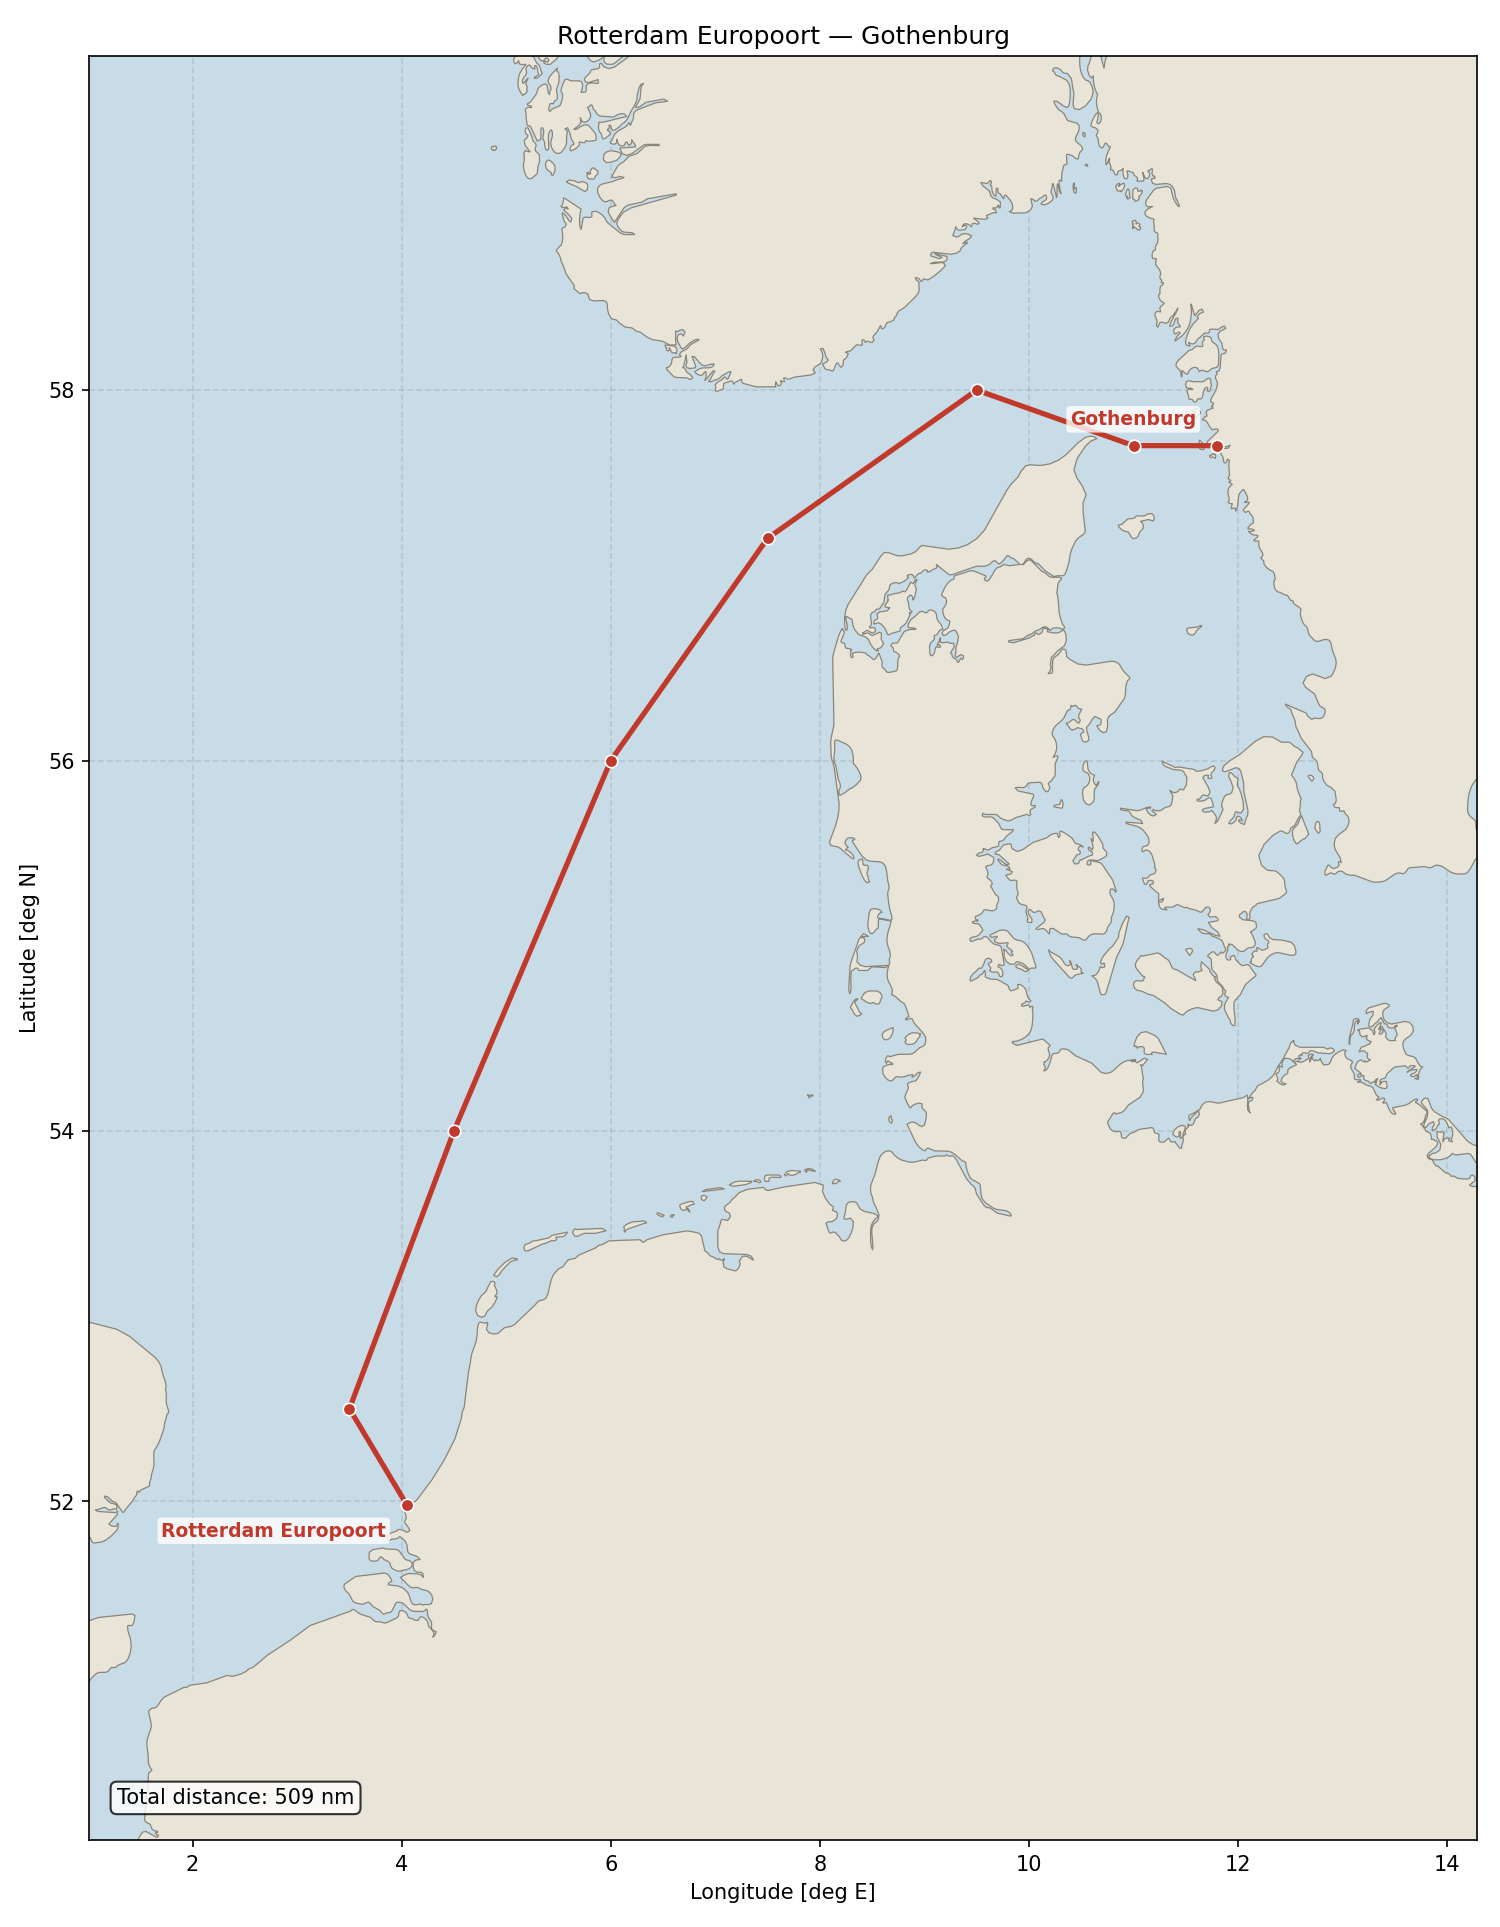
\includegraphics[width=0.85\textwidth]{voyage_comparison_route.png}
\caption{Rotterdam--Gothenburg route (509 nm one-way) with waypoints and leg bearings.  Coastline data from Natural Earth 10m.}
\end{figure}

\subsection{Voyage Statistics}
\label{sec:org9b86b57}

362 round-trip voyages were successfully simulated (4 late-December departures
failed due to missing January 2025 weather data).

\begin{center}
\begin{tabular}{lrrrrrr}
\toprule
Metric & Mean & Median & P10 & P90 & Min & Max\\[0pt]
\midrule
Factory no-Fl [kg/voy] & 17271 & 17062 & 16107 & 18996 & 12980 & 22239\\[0pt]
Opt + Flettner [kg/voy] & 15000 & 15043 & 12865 & 16959 & 10253 & 20844\\[0pt]
Pitch/RPM saving [kg/voy] & 899 & 929 & 794 & 970 & 462 & 998\\[0pt]
Flettner saving [kg/voy] & 1372 & 1208 & 331 & 2719 & 8 & 4942\\[0pt]
Pitch/RPM saving & 5.2\% & 5.4\% & 4.2\% & 5.9\% & 2.6\% & 6.4\%\\[0pt]
Flettner saving & 8.0\% & 6.9\% & 2.0\% & 16.1\% & 0.0\% & 28.9\%\\[0pt]
Mean \(H_s\) [m] & 1.4 & 1.3 & 0.7 & 2.3 & 0.4 & 4.0\\[0pt]
Mean wind speed [m/s] & 7.8 & 7.6 & 5.3 & 10.6 & 3.5 & 14.5\\[0pt]
Mean \(R_\text{aw}\) [kN] & 4.7 & 2.1 & 0.2 & 12.4 & -0.9 & 45.2\\[0pt]
Mean \(R_\text{wind}\) [kN] & 4.5 & 4.0 & -0.6 & 10.5 & -4.5 & 26.9\\[0pt]
Mean Flettner thrust [kN] & 14.3 & 11.5 & 3.2 & 30.5 & 0.1 & 55.7\\[0pt]
Mean rotor power [kW] & 17.4 & 13.9 & 4.0 & 37.6 & 0.2 & 68.0\\[0pt]
\bottomrule
\end{tabular}
\end{center}

Fuel savings are decomposed additively against the factory-no-Flettner baseline:

\begin{equation}
  \underbrace{\text{Factory}_\text{NF} - \text{Opt}_\text{+Fl}}_{\text{combined saving}}
  = \underbrace{\text{Factory}_\text{NF} - \text{Opt}_\text{NF}}_{\text{pitch/RPM}}
  + \underbrace{\text{Opt}_\text{NF} - \text{Opt}_\text{+Fl}}_{\text{Flettner}}
\end{equation}

The pitch/RPM saving (5.2\%) isolates the benefit of optimising the
operating point at the same thrust demand.  The Flettner saving (7.9\%)
isolates the thrust reduction from the rotor.  Both percentages are relative to
the factory-no-Flettner baseline.

Figure \ref{fig:org82dac97} shows the daily evolution of fuel savings, significant
wave height, and force components across the full year.

\begin{figure}[H]
\centering
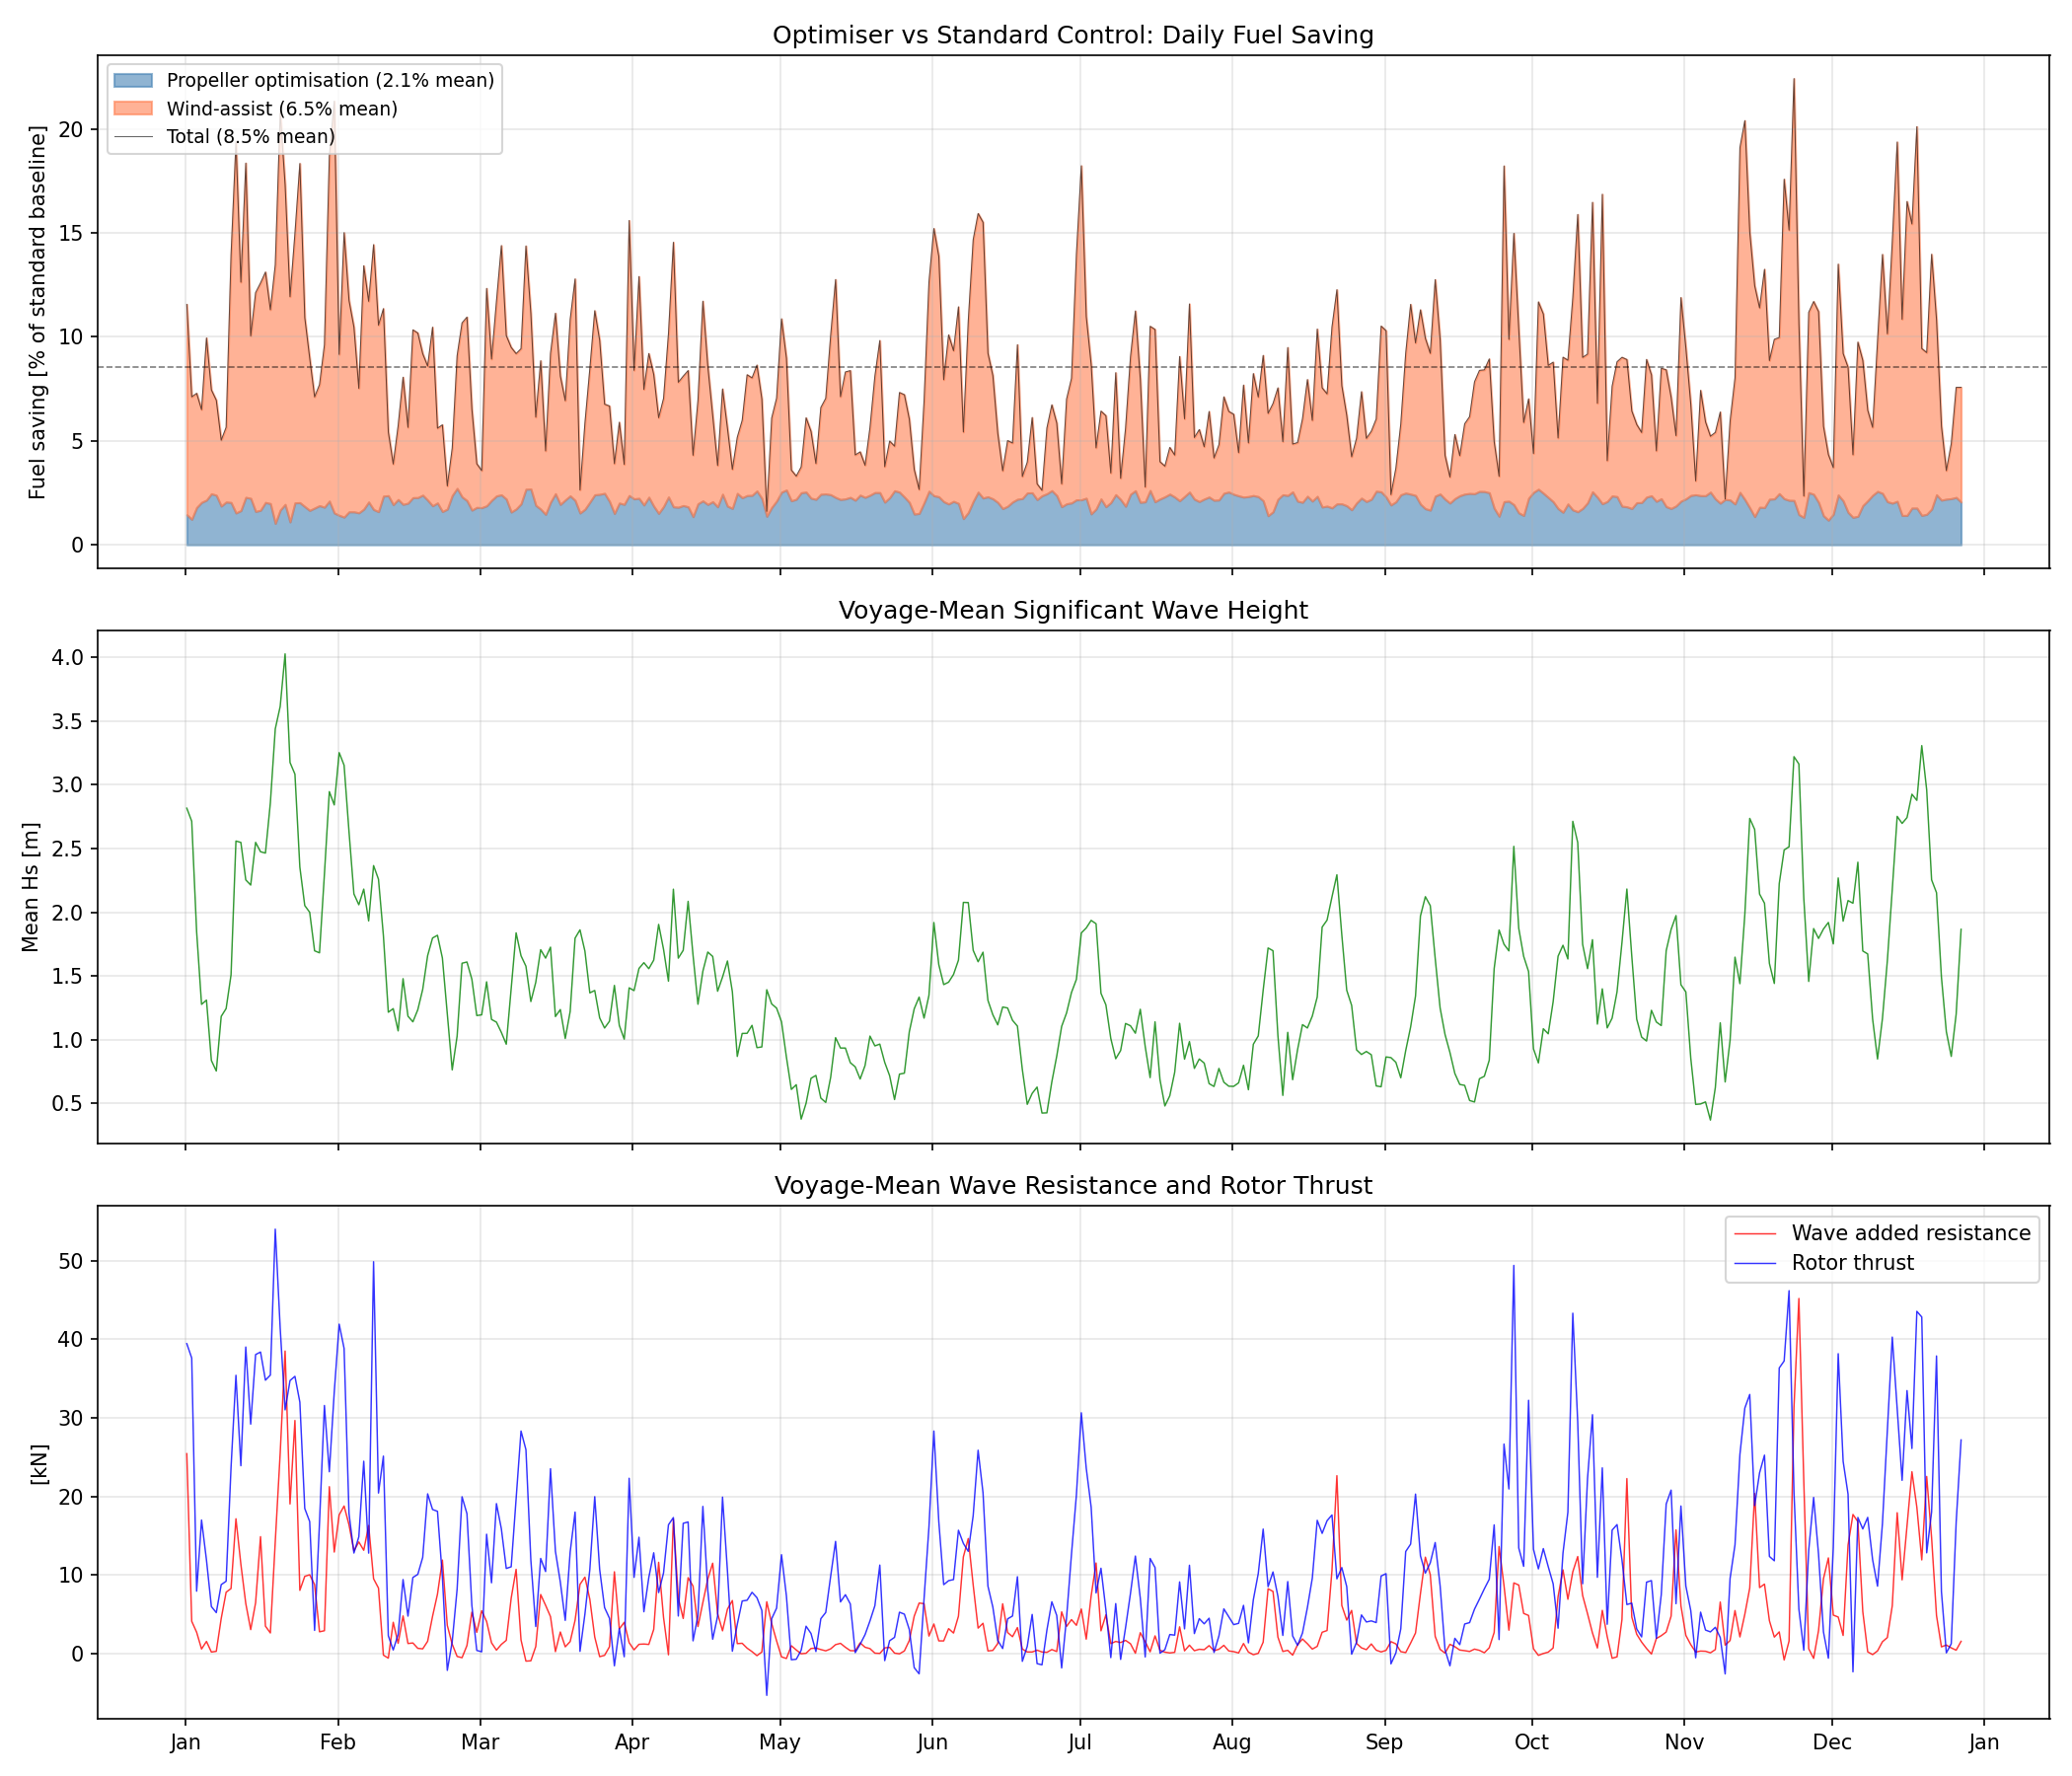
\includegraphics[width=\textwidth]{voyage_comparison_results.png}
\caption{\label{fig:org82dac97}Annual time-series of per-voyage results.  Top: pitch/RPM and Flettner fuel savings (stacked).  Middle: significant wave height.  Bottom: added wave resistance, wind resistance, and Flettner thrust.}
\end{figure}

\subsection{Factory Combinator Feasibility}
\label{sec:org24c4702}

\begin{center}
\begin{tabular}{lr}
\toprule
Metric & Value\\[0pt]
\midrule
Total evaluation hours & 37\thinspace648\\[0pt]
Both feasible & 98\%\\[0pt]
Factory infeasible hours & 0\%\\[0pt]
Voyages with \(\geq 1\) infeasible hour & 7\%\\[0pt]
\bottomrule
\end{tabular}
\end{center}

Factory infeasibility occurs when the engine exceeds its power envelope at the
factory combinator's fixed RPM schedule.  The optimiser adapts pitch/RPM to
remain feasible.

Figure \ref{fig:org3b55e65} shows the correlation between per-voyage fuel saving and
mean sea state, coloured by mean wind speed.  Higher seas drive larger absolute
savings through the Flettner rotor.

\begin{figure}[H]
\centering
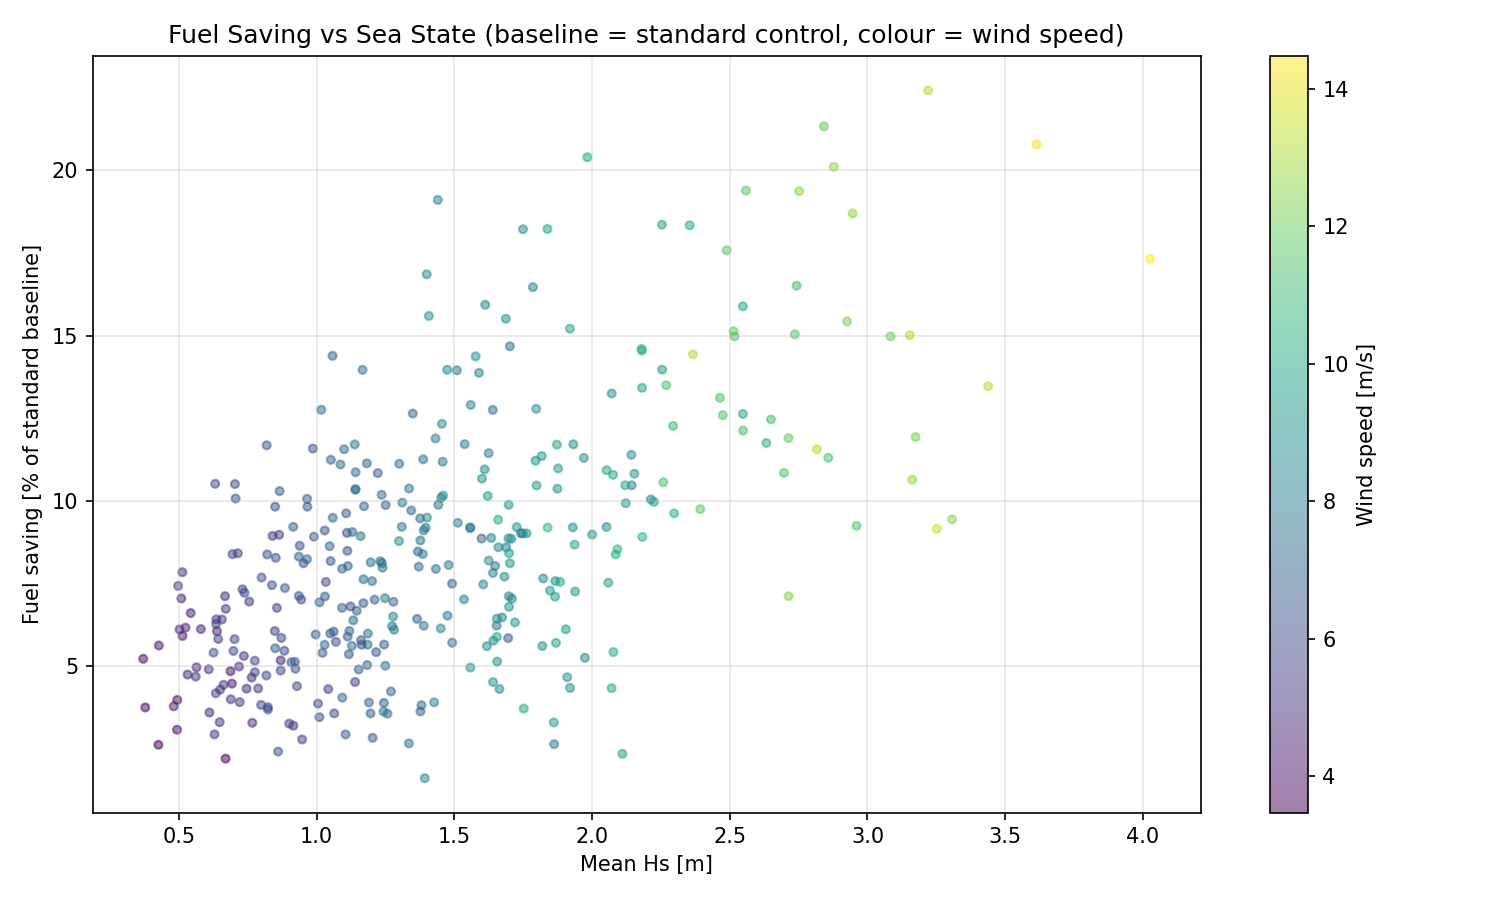
\includegraphics[width=0.85\textwidth]{voyage_comparison_scatter.png}
\caption{\label{fig:org3b55e65}Per-voyage fuel saving vs mean significant wave height, coloured by mean wind speed.  The positive correlation reflects the Flettner rotor's increasing benefit in windier conditions.}
\end{figure}

\subsection{Annualised Fuel Consumption}
\label{sec:orgbadcc38}

Assuming 15\% idle time, the vessel completes approximately 73 round-trip
voyages per year.

\begin{center}
\begin{tabular}{lr}
\toprule
Configuration & Fuel [tonnes/year]\\[0pt]
\midrule
Factory, no Flettner & 1262.9\\[0pt]
Factory + Flettner & 1161.8\\[0pt]
Optimiser, no Flettner & 1197.2\\[0pt]
Optimiser + Flettner & 1096.9\\[0pt]
\bottomrule
\end{tabular}
\end{center}

\begin{center}
\begin{tabular}{lrr}
\toprule
Saving component & Tonnes/year & Percentage\\[0pt]
\midrule
Pitch/RPM & 65.7 & 5.2\%\\[0pt]
Flettner & 100.3 & 7.9\%\\[0pt]
Combined & 166.1 & 13.1\%\\[0pt]
\bottomrule
\end{tabular}
\end{center}

Figure \ref{fig:org3ebc472} shows the distribution of per-voyage savings, decomposed
into pitch/RPM optimisation and Flettner wind-assist components.

\begin{figure}[H]
\centering
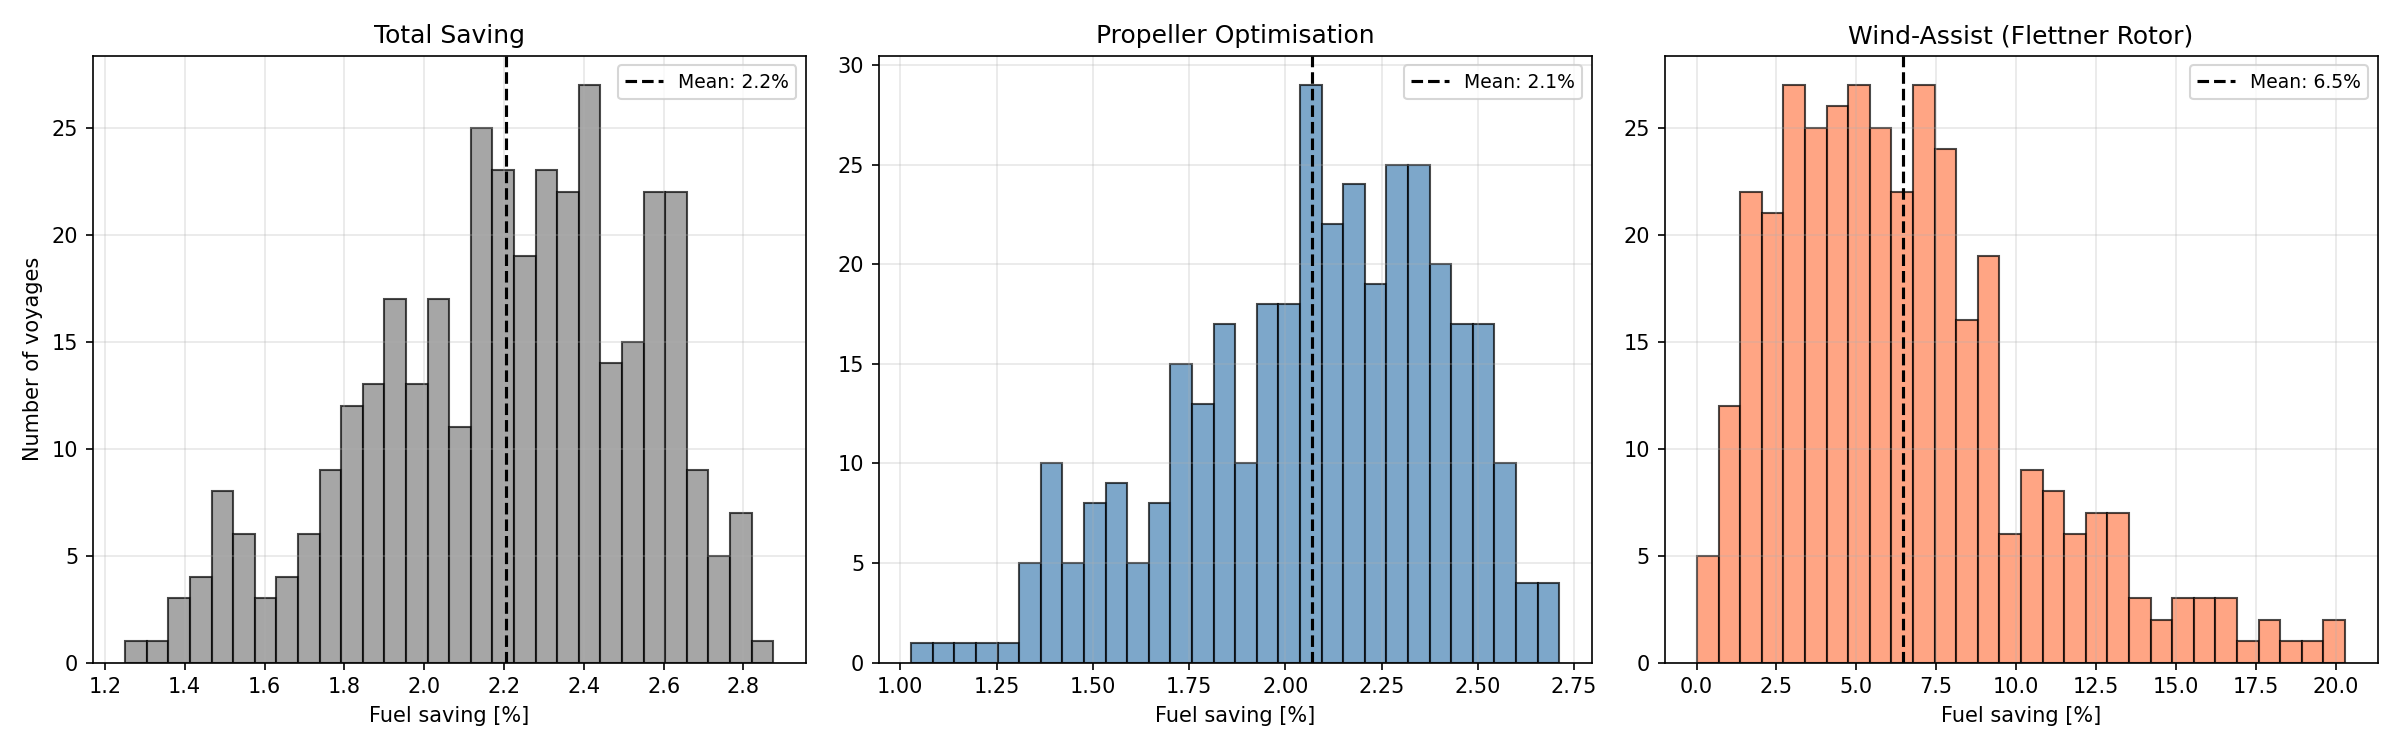
\includegraphics[width=\textwidth]{voyage_comparison_histogram.png}
\caption{\label{fig:org3ebc472}Histograms of per-voyage fuel savings.  Left: total saving (factory vs optimiser+Flettner).  Centre: pitch/RPM component.  Right: Flettner component.  The Flettner saving has a wider spread reflecting its weather dependence.}
\end{figure}

\subsection{Cost Estimates}
\label{sec:orgf17b17f}

At MGO price of \euro650/tonne (typical ECA zone):

\begin{center}
\begin{tabular}{lr}
\toprule
Configuration & Annual cost\\[0pt]
\midrule
Factory, no Flettner & \euro820\thinspace911\\[0pt]
Factory + Flettner & \euro755\thinspace157\\[0pt]
Optimiser, no Flettner & \euro778\thinspace194\\[0pt]
Optimiser + Flettner & \euro712\thinspace970\\[0pt]
Annual saving & \euro107\thinspace941 (13.1\%)\\[0pt]
\bottomrule
\end{tabular}
\end{center}

\subsection{Seasonal Breakdown}
\label{sec:org545b276}

\begin{center}
\begin{tabular}{lrrrrrrr}
\toprule
Season & Voyages & Fac NF [kg] & Opt+Fl [kg] & Saving & P/R & Flettner & Mean \(H_s\) [m]\\[0pt]
\midrule
Q1 (Jan--Mar) & 91 & 17\thinspace327 & 14\thinspace731 & 5.4\% & 5.0\% & 10.1\% & 1.8\\[0pt]
Q2 (Apr--Jun) & 91 & 17\thinspace315 & 15\thinspace378 & 5.8\% & 5.4\% & 5.9\% & 1.2\\[0pt]
Q3 (Jul--Sep) & 92 & 17\thinspace181 & 15\thinspace206 & 5.8\% & 5.4\% & 6.1\% & 1.1\\[0pt]
Q4 (Oct--Dec) & 88 & 17\thinspace261 & 14\thinspace671 & 5.5\% & 5.1\% & 10.1\% & 1.7\\[0pt]
\bottomrule
\end{tabular}
\end{center}

The Flettner benefit is roughly doubled in the winter quarters (Q1, Q4) compared
to summer, reflecting the stronger and more consistent North Sea wind regime.
The pitch/RPM optimisation saving is relatively stable across seasons at
5.0--5.4\%, as it depends primarily on the thrust demand distribution rather than
its magnitude.

\subsection{Shaft Generator Mode}
\label{sec:orgf287506}

The preceding results assume the vessel operates without a shaft generator (SG).
When the SG is online, two additional constraints apply:

\begin{enumerate}
\item \textbf{Parasitic load:} The SG extracts electrical power from the main engine shaft,
increasing total engine load.  A typical average SG load of \SI{150}{\kilo\watt}
is assumed.

\item \textbf{RPM floor:} The SG must maintain output frequency within the permitted band
(\SIrange{48}{60}{\hertz}).  At the PTO gear ratio, this constrains the minimum
engine RPM to approximately \SI{640}{RPM} (shaft RPM \(\geq\) \SI{94.1}{RPM}).
\end{enumerate}

Both constraints apply equally to the factory combinator and the optimiser.  The
factory combinator schedule is constructed with \SI{200}{\kilo\watt} SG headroom
(the margin the hydrodynamicist uses when designing the combinator, on top of the
standard \SI{300}{\kilo\watt} between the propeller curve and the torque limit),
while the actual SG load of \SI{150}{\kilo\watt} is used in the fuel evaluation
for both factory and optimiser.

\begin{verbatim}
python voyage_comparison.py --year 2024 --speed 10 --quiet \
    --sg-load 150 --sg-factory-allowance 200 \
    --sg-freq-min 48 --sg-freq-max 60
\end{verbatim}

\subsubsection{Annualised Fuel (SG Mode)}
\label{sec:orged36cc5}

\begin{center}
\begin{tabular}{lr}
\toprule
Configuration & Fuel [tonnes/year]\\[0pt]
\midrule
Factory, no Flettner & 1513.9\\[0pt]
Factory + Flettner & 1414.9\\[0pt]
Optimiser, no Flettner & 1437.7\\[0pt]
Optimiser + Flettner & 1332.0\\[0pt]
\bottomrule
\end{tabular}
\end{center}

\begin{center}
\begin{tabular}{lrr}
\toprule
Saving component & Tonnes/year & Percentage\\[0pt]
\midrule
Pitch/RPM & 76.3 & 5.0\%\\[0pt]
Flettner & 105.7 & 7.0\%\\[0pt]
Combined & 182.0 & 12.0\%\\[0pt]
\bottomrule
\end{tabular}
\end{center}

\subsubsection{Interpretation}
\label{sec:org95b0c06}

With the corrected hull data (model test trial prediction), the calm-water
thrust demand at \SI{10}{\knot} is approximately \SI{133}{\kilo\newton},
requiring shaft power of approximately \SI{767}{\kilo\watt} and shaft RPM
\(\approx 75\).  Even with the SG RPM floor at \SI{94.1}{RPM}, the factory
combinator schedule is built with the SG headroom, so its operating points
differ from the optimiser's.  The higher resistance means the engine operates
well above the SG RPM floor for much of the voyage, giving the optimiser room to
select a better pitch/RPM combination.

The pitch/RPM saving is 5.0\%, comparable to the 5.2\% in
standard mode.  The Flettner saving is 7.0\%.

At \SI{10}{\knot} the SG constraint does not significantly affect savings with
the corrected hull data.  The speed sweep under SG constraints was not re-run
with the updated hull data; however, at \SI{10}{\knot} the results are:

\begin{center}
\begin{tabular}{lrrrrr}
\toprule
Speed & Pitch/RPM saving & Flettner saving & Combined saving & Annual saving\\[0pt]
\midrule
\SI{10}{\knot} & 5.0\% & 7.0\% & 12.0\% & \euro118k\\[0pt]
\bottomrule
\end{tabular}
\end{center}

\subsubsection{SG vs Auxiliary Genset Fuel Efficiency}
\label{sec:org3153ccf}

An important question is whether the shaft generator is the most fuel-efficient
way to supply \SI{150}{\kilo\watt} of electrical power.  The alternative is a
separate auxiliary diesel genset.

With the SG on the main engine, the factory combinator burns \SI{1514}{t/yr}.
Without the SG, it burns \SI{1263}{t/yr} --- a difference of \SI{251}{t/yr}.
This incremental fuel for \SI{150}{\kilo\watt} over \SI{7439}{h/yr} corresponds
to an \emph{effective} SFOC of \SI{225}{\gram/\kilo\watt\hour}.

This is only slightly worse than a typical auxiliary genset (\SI{210}--\SI{230}{\gram/\kilo\watt\hour}).
With the corrected hull data, the engine operates at higher load even at
\SI{10}{\knot}, reducing the RPM floor penalty.  The effective SFOC is close to
the genset range, making the SG vs genset choice marginal at this speed.

The breakeven genset SFOC --- the value at which a separate genset becomes
more expensive than running the SG on the ME --- is \SI{225}{\gram/\kilo\watt\hour}
for the factory combinator.  At a genset SFOC of \SI{215}{\gram/\kilo\watt\hour},
a separate auxiliary genset saves approximately \SI{11}{t/yr}
(\euro7k/yr) compared to the SG --- a much smaller margin than
previously estimated.

At higher speeds the picture changes: the RPM constraint penalty diminishes
further, and the ME's superior part-load SFOC makes the SG more competitive.

\subsubsection{Cost Estimates (SG Mode)}
\label{sec:org4776992}

At MGO \euro650/tonne:

\begin{center}
\begin{tabular}{lr}
\toprule
Configuration & Annual cost\\[0pt]
\midrule
Factory, no Flettner & \euro984\thinspace050\\[0pt]
Optimiser + Flettner & \euro865\thinspace769\\[0pt]
Annual saving & \euro118\thinspace281 (12.0\%)\\[0pt]
\bottomrule
\end{tabular}
\end{center}

\subsubsection{Seasonal Breakdown (SG Mode)}
\label{sec:orge634c4d}

\begin{center}
\begin{tabular}{lrrrrrrr}
\toprule
Season & Voyages & Fac NF [kg] & Opt+Fl [kg] & Saving & P/R & Flettner & Mean \(H_s\) [m]\\[0pt]
\midrule
Q1 (Jan--Mar) & 91 & 20\thinspace713 & 17\thinspace886 & 5.9\% & 4.9\% & 8.9\% & 1.8\\[0pt]
Q2 (Apr--Jun) & 91 & 20\thinspace728 & 18\thinspace587 & 5.9\% & 5.2\% & 5.2\% & 1.2\\[0pt]
Q3 (Jul--Sep) & 92 & 20\thinspace581 & 18\thinspace400 & 5.9\% & 5.3\% & 5.4\% & 1.1\\[0pt]
Q4 (Oct--Dec) & 88 & 20\thinspace794 & 17\thinspace975 & 6.0\% & 4.9\% & 8.8\% & 1.7\\[0pt]
\bottomrule
\end{tabular}
\end{center}

\subsubsection{Summary Comparison: Standard vs SG Mode}
\label{sec:org445c8fe}

\begin{center}
\begin{tabular}{lrr}
\toprule
Metric & Standard mode & SG mode (150 kW)\\[0pt]
\midrule
Baseline fuel [t/yr] & 1262.9 & 1513.9\\[0pt]
Pitch/RPM saving & 5.2\% (66 t/yr) & 5.0\% (76 t/yr)\\[0pt]
Flettner saving & 7.9\% (100 t/yr) & 7.0\% (106 t/yr)\\[0pt]
Combined saving & 13.1\% (166 t/yr) & 12.0\% (182 t/yr)\\[0pt]
Annual cost saving & \euro108k & \euro118k\\[0pt]
\bottomrule
\end{tabular}
\end{center}

The choice of whether to operate with the SG has a modest impact on savings.
When the SG is offline, the Optimiser saves 5.2\% from pitch/RPM
optimisation.  When the SG is online, the higher resistance from the corrected
hull data means the engine operates well above the RPM floor, preserving most of
the optimiser's freedom --- the pitch/RPM saving is 5.0\%.  The
Flettner rotor remains beneficial in both cases with similar relative impact.

The effective SFOC of the main engine for the SG load is \SI{225}{\gram/\kilo\watt\hour},
close to a typical auxiliary genset (\SI{215}{\gram/\kilo\watt\hour}).  At
\SI{10}{\knot} transit speed, a separate genset is only marginally more
fuel-efficient than the shaft generator, saving approximately \SI{11}{t/yr}
(\euro7k/yr).

Figure \ref{fig:orgd4cbca2} shows the side-by-side comparison of daily fuel
savings in standard and SG modes.

\begin{figure}[H]
\centering
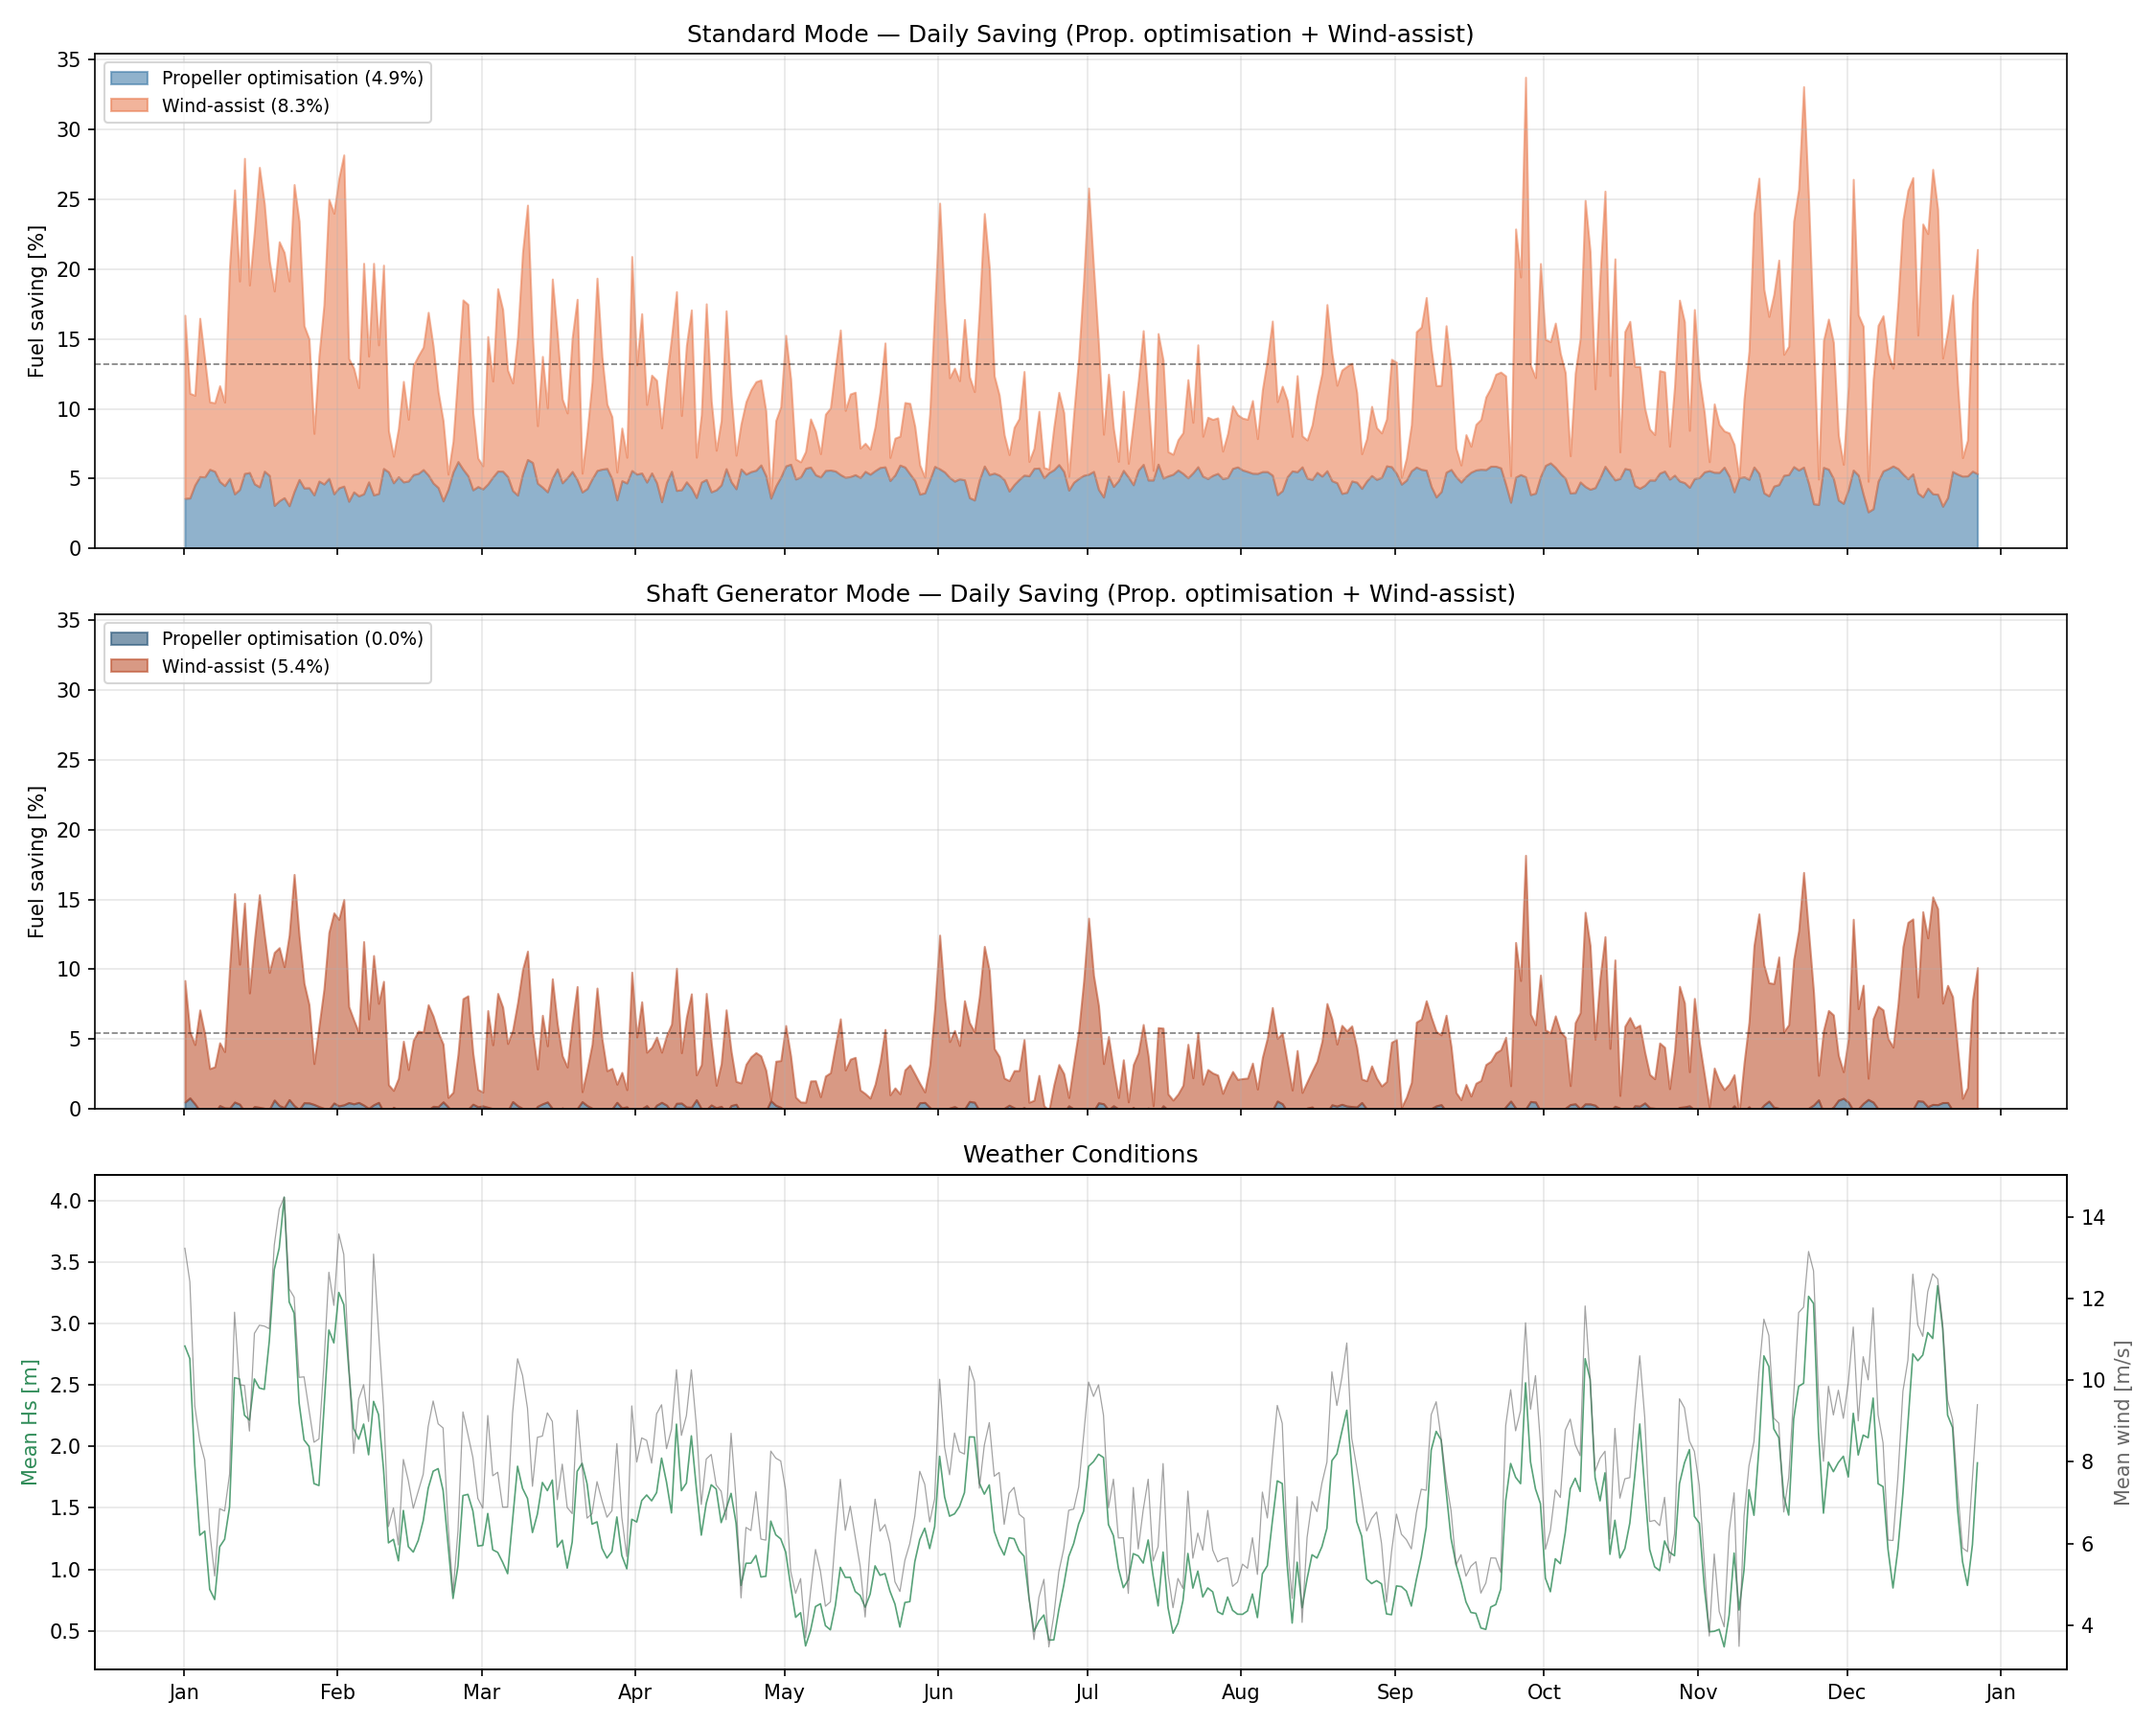
\includegraphics[width=\textwidth]{comparison_timeseries.png}
\caption{\label{fig:orgd4cbca2}Side-by-side comparison of daily fuel savings in standard mode (top) vs shaft generator mode (bottom).  With the corrected hull data, the pitch/RPM saving is preserved in SG mode, and the Flettner benefit remains comparable.}
\end{figure}

\section{Conclusions}
\label{sec:org78b6b83}

The refactored \texttt{voyage\_comparison} tool has been validated by running a
full-year (2024) hindcast simulation on the Rotterdam--Gothenburg route.  Key
findings:

\begin{enumerate}
\item \textbf{Standard mode (SG offline):} Pitch/RPM optimisation saves \textbf{5.2\%}
(66 t/yr, \euro43k/yr); Flettner wind-assist adds \textbf{7.9\%}
(100 t/yr, \euro65k/yr); combined \textbf{13.1\%}
(166 t/yr, \euro108k/yr) at \SI{10}{\knot}.

\item \textbf{SG mode (150 kW, 48--60 Hz):} With the corrected hull data (higher
resistance), the engine operates well above the SG RPM floor even at
\SI{10}{\knot}, preserving most of the optimiser's freedom.  Pitch/RPM saving
is \textbf{5.0\%} (76 t/yr).  Flettner retains \textbf{7.0\%}
(106 t/yr).  Combined saving \textbf{12.0\%} (182 t/yr,
\euro118k/yr).  The effective SFOC of the main engine for the SG
load is \SI{225}{\gram/\kilo\watt\hour} --- close to a typical auxiliary
genset at \SI{215}{\gram/\kilo\watt\hour} --- making the SG vs genset
trade-off marginal at \SI{10}{\knot}.  A separate genset saves approximately
\SI{11}{t/yr} (\euro7k/yr).

\item The factory combinator becomes \textbf{infeasible} (engine over-power) on 7\% of
voyages, while the optimiser adapts pitch/RPM to remain within the power
envelope.

\item The \textbf{modular architecture} (4 packages, 24 modules, 5\thinspace181 lines)
provides clean separation of physical models, simulation logic, reporting, and
visualisation, enabling independent testing and extension of each component.
\end{enumerate}

\section{References}
\label{sec:org05eef08}

\begin{itemize}
\item Blendermann, W. (1994). Parameter identification of wind loads on ships.
\emph{J. Wind Eng. Ind. Aerodyn.}, 51(3), 339--351.
\item Bordogna, G., Muggiasca, S., Giappino, S., Belloli, M., Keuning, J.A.,
Huijsmans, R.H.J. (2019). The effects of the aerodynamic interaction on the
performance of two Flettner rotors. \emph{J. Wind Eng. Ind. Aerodyn.}, 196, 104024.
\item Mosaad, M.A. (1986). Marine propeller roughness penalties. PhD Thesis,
University of Newcastle upon Tyne.
\item Theodorsen, T. \& Regier, A. (1944). Experiments on drag of revolving disks,
cylinders, and streamline rods at high speeds. \emph{NACA Report 793}.
\item Townsin, R.L. \& Dey, S.K. (2003). The correlation of roughness drag with
surface characteristics. In \emph{Biofouling}, Royal Institution of Naval Architects.
\end{itemize}
\end{document}
